\section*{Trusted Path}

Although SGX enclaves provide a notion of \emph{secure computation}, they do not easily lend themselves to \emph{secure user interaction}. The main reason for this is that, in an architecture like SGX, enclaves communicate with I/O devices through the untrusted OS. When an enclave needs to receive user input, it is the responsibility of the OS to pass data from an input device like keyboard or mouse to the enclave. When an enclave needs to send user output, it is the responsibility of the OS to forward output data received from the enclave to a user output device like the screen. Such TEE design means that a compromised OS can trivially modify any user input and output and read any secrets that are communicated between the user and the enclave. 

Such user input and output manipulation can have severe consequences in several application scenarios. For example, if a malicious OS modified user input that is provided to a financial enclave, the enclave could be tricked to perform unauthorized payments. If enclaves are used to control safety-critical system such as a medical devices or industrial systems, user input modifications may cause serious safety risks. Also any enclave that needs to be configured with a password or similar user authentication credential is difficult to implement securely in an architecture like SGX.

Such lack of secure user interaction capabilities means that SGX-style enclaves do not support \emph{trusted path}. Two types of trusted paths are possible. The first, and more common, definition of trusted path is a secure communication channel between the human user and a \emph{local} application like an enclave. The second, and perhaps less common, definition of trusted path is one that realizes a secure communication channel between the user and the remote server. In this section of the article, we... 


\subsubsection*{Requirements}
\label{goals}

The lack of security properties and features in the existing solutions provides the necessary security and functional requirements for a trusted path that provides IO integrity and confidentiality and is usable. 

\paragraph{R1. Inter-dependency between input and output} 
IntegriKey~\cite{IntegriKey} use external embedded devices to sign input parameters. However, such solutions do not support output integrity; hence, the attacker can execute UI manipulation attacks to trick the user into providing incorrect inputs. Such observation shows that the output and input security depend on each other, and they should be considered together. Otherwise, the attacker can manipulate the output to influence the user input.
%The main lesson that we learn from the previous papers is that input and output integrity, and confidentiality cannot be considered in isolation. Rather, they are needed to be secured simultaneously as the output, and the input both influence each other.  

\paragraph{R2. Inter-dependency between all input modalities} 
Fidelius~\cite{Fidelius} combines the previous ideas of Bump in the Ether and trusted overlay to protect keyboard inputs from a compromised browser using external devices and a JavaScript interpreter that runs inside an SGX enclave. However, not supporting mouse causes Fidelius to susceptible to early form submission attack where the attacker could maliciously submit a form when the user is still typing - violation of input integrity. Existing web interfaces allow users to complete forms by using different modalities for the user input, namely the keyboard, the mouse, and the touchpad. The observation from Fidelius secure shows that system should protect simultaneously all user input modalities to achieve input integrity (against early-form submission and clickjacking).


\paragraph{R3a. No cognitive load for IO integrity} 
A system that protects IO operations should introduce minimal or no cognitive load to its users for input integrity.
The system should guarantee the output integrity of the legitimate information necessary to complete a form and avoid asking the user to interact with an external device or monitor security indicators out-of-context.




\subsubsection*{Description of \name}

\begin{figure}[t]
	\centering
	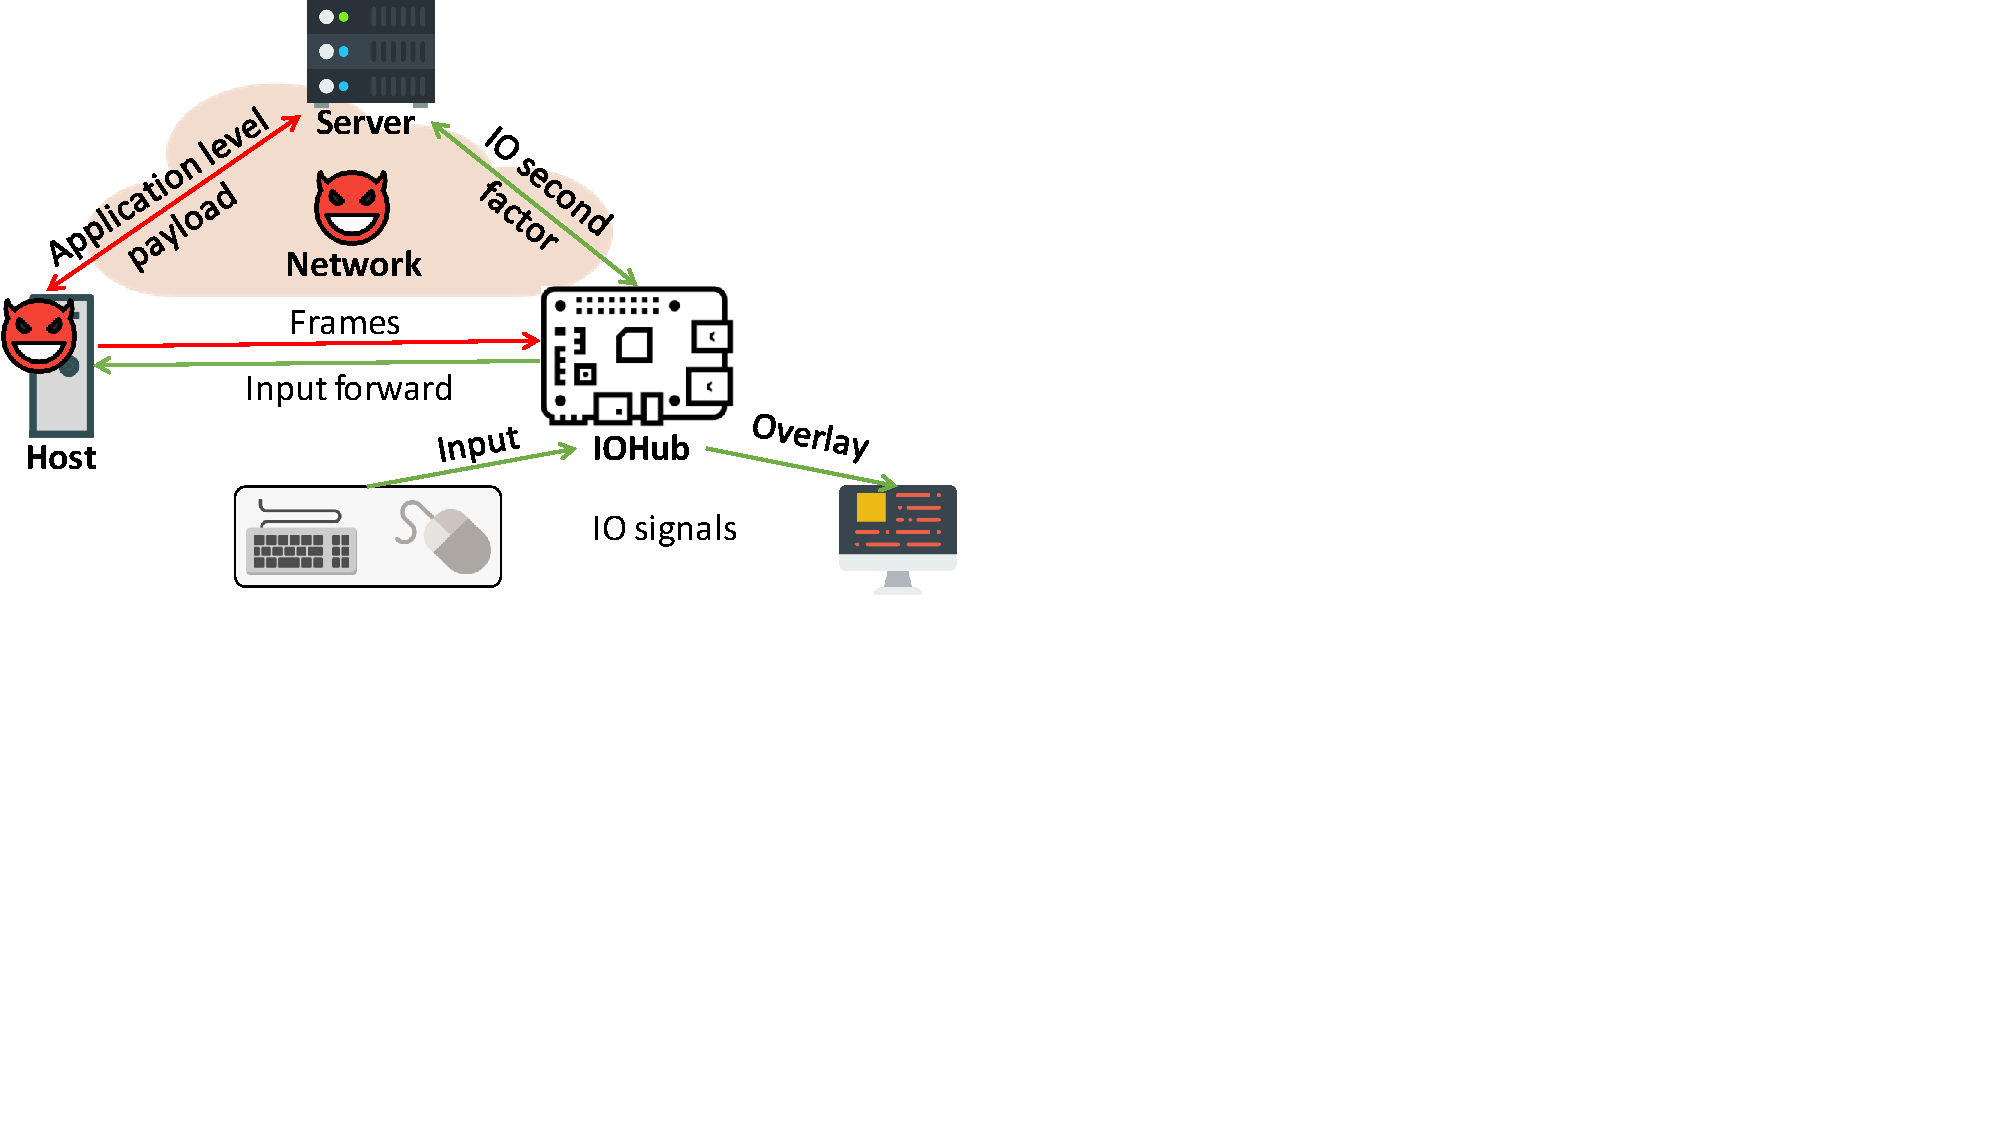
\includegraphics[trim={0 8.5cm 17cm 0}, clip, width=0.9\linewidth]{approachOverview.pdf}
	\caption{High-level approach overview of our solution.  The \device connects the trusted IO devices and the attacker-controlled host.}
	\label{fig:approachOverview}
\end{figure}

The model is depicted in Figure~\ref{fig:approachOverview} which shows the untrusted host, the remote server, and the user IO devices. We only assume that the monitor, keyboard, mouse (in a word all the IO devices that we need to protect from the malicious host) and the \device are trusted. The \device works as a mediator between all the IO devices and the host. Note that the \device has no network capability to communicate with the server directly, rather it relies on the host and uses it as an untrusted transport. We also assume that the \device comes with preloaded certificates and keys that allow the \device to verify the signatures signed by the server and sign data such as the user input.

There are many possible ways to deploy \name. One way is to assume that the \device manufacturer issues a certificate for each of the deployed \device{}s . The \device maintains a whitelist for the remote servers along with their public certificates. This allows the \device to verify messages signed by those remote servers. Another assumption could be that the \device is issued by a service provider who also runs the remote server. 

\name is build upon the security requirements and functional properties that are described in Section~\ref{goals}. 
\device is active only when the user visits sensitive web applications that require \name security.
Initially, the remote server signs and delivers the sensitive UI elements to the host in a format that is understandable by \device. Next, the host transfers the sensitive UI to \device, and the \device verifies the signature to prevent manipulations by the host. As seen in a running example depicted in Figure~\ref{fig:screenshot_1}, the \device then renders the UI with sensitive elements into an overlay on top of the HDMI frame received from the host. Note that the host cannot access or modify the overlay generated by the \device. Also, the overlay covers only a part of the screen, allowing the other feature-rich content on the webpage to run unmodified. Therefore, this ensures that sensitive UI elements are presented to the user as expected by the remote server -- \emph{output integrity}. For the overlay, we use QR-codes to transfer data from the host to the device because we avoid using extra software/hardware for a separate channel, and it is easy to visualize.

\begin{figure*}[t]
	\centering
	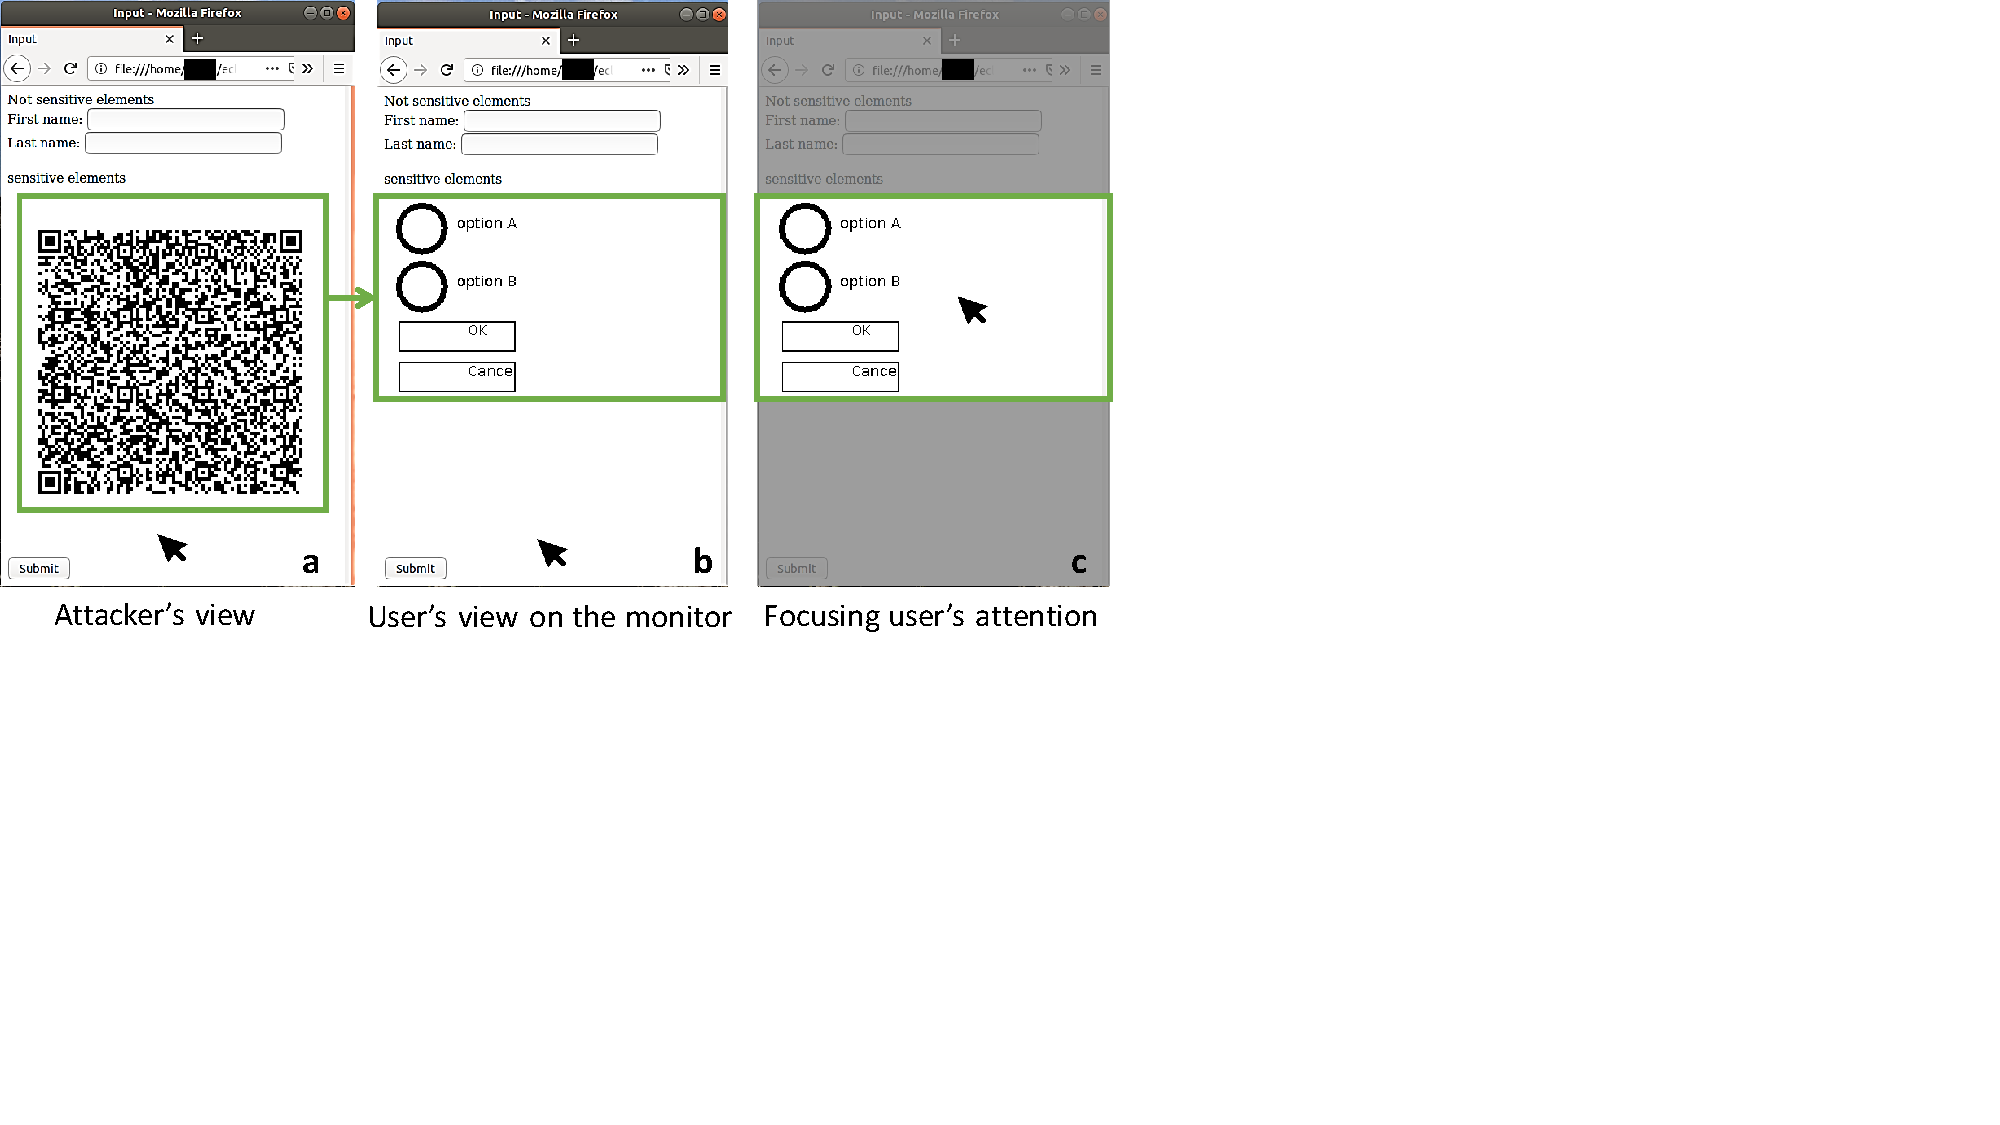
\includegraphics[trim={0 8cm 15cm 0}, clip, width=0.6\linewidth]{overlayScreenShot_new.pdf}
	\caption{\name's high-level approach shows that the \device generates UI overlay to protect IO integrity and confidentiality.}
	\label{fig:screenshot_1}
\end{figure*}

When the user interacts (types or moves the pointer) with the overlay, \device does not forward any event from the keyboard or the mouse to the host. The interaction is maintained solely by \device, which renders on-screen user inputs and therefore offers a user experience that is identical to a typical one as if the \device is not present. The user click on the \emph{submit} button triggers the submission procedure, which consists of the \device signing the user inputs and sending to the server. Note that the text fields of the form and the \emph{submit} button are inside the overlay which is inaccessible by the host, hence the attacker cannot execute the early form submission or clickjacking attacks. Finally, the server verifies the signature of \device to guarantee that the host has not altered the data. Therefore, the \device ensures \emph{input integrity} for all \emph{modalities} of input.

For integrity guarantees, \name uses well-known user attention focusing mechanisms such as lightbox that aid the user to distinguish the \device overlay on the screen from the rest. Thus, the untrusted host cannot trick the user into following malicious instructions when the user interacts with sensitive UI elements. Also, the host cannot observe sensitive data on the overlay because it does not have access to it. In the case where confidentiality is required, the user manually triggers SAS, such as the lightbox by pressing specific keys.


\begin{figure}[t]
	\centering
	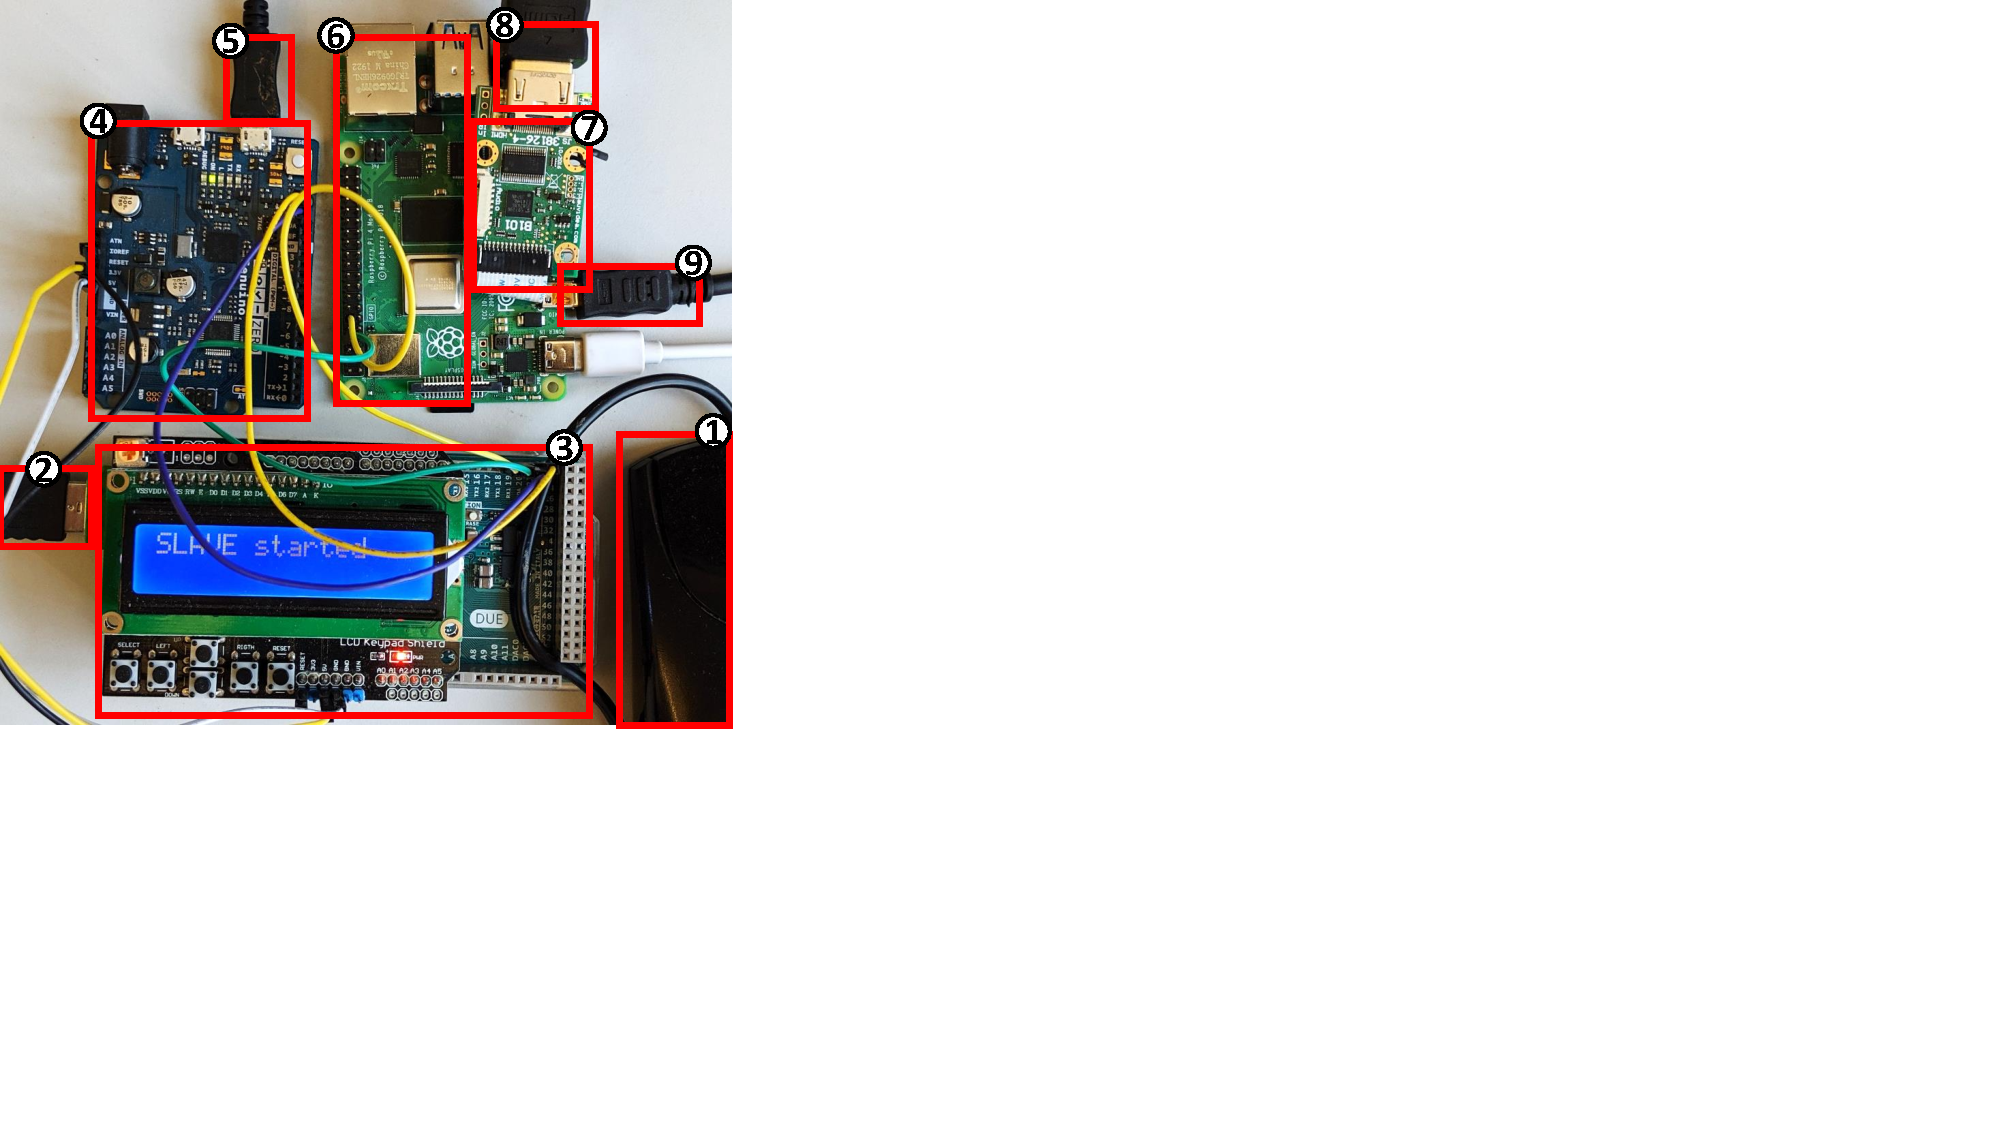
\includegraphics[trim={0 6.6cm 21.5cm 0}, clip, scale=0.5]{setUp_1.pdf}
	\caption{The figure shows \name prototype.}
\label{fig:prototypeArch}   
\end{figure}

\subsubsection*{Prototype}

Figure~\ref{fig:prototypeArch} shows our \device prototype.
The delay in forwarding keystrokes is $170\ \mu s$ and for frames is $21.76\ ms$. This allows the \device to achieve the maximum display frame rate of $47.69$ per second (e.g., most of the movies are shot and shown in  ~24-30 fps).






